\documentclass{scrartcl}
\pagestyle{empty}

\usepackage{graphicx}
\usepackage{tikz}
\usetikzlibrary{arrows}

\usepackage[margin=0cm]{geometry}


\newcommand{\imgSize}{.2\textwidth}
\newcommand{\descrTextWidth}{4cm}

% ----------------------
\begin{document}
\begin{figure}
\begin{center}



\begin{tikzpicture}


% Insert all the pictures
\node[inner sep=0pt] (lotShuffle) at (0,0)
    {
\includegraphics[width=\imgSize]{lotShuffle.jpg}};

\node[inner sep=0pt] (trialCount) at (0,-4)
    {
\includegraphics[width=\imgSize]{spCounter.jpg}};    

\node[inner sep=0pt] (fixcross) at (0,-8)
    {
\includegraphics[width=\imgSize]{fixcross.jpg}};
    
\node[inner sep=0pt] (outcome) at (0,-12)
    {
\includegraphics[width=\imgSize]{outBlueRight.jpg}};
 
\node[inner sep=0pt] (earn) at (0,-16)
    {
\includegraphics[width=\imgSize]{earnZero.jpg}}; 
   
\node[inner sep=0pt] (prefLot) at (0,-20)
    {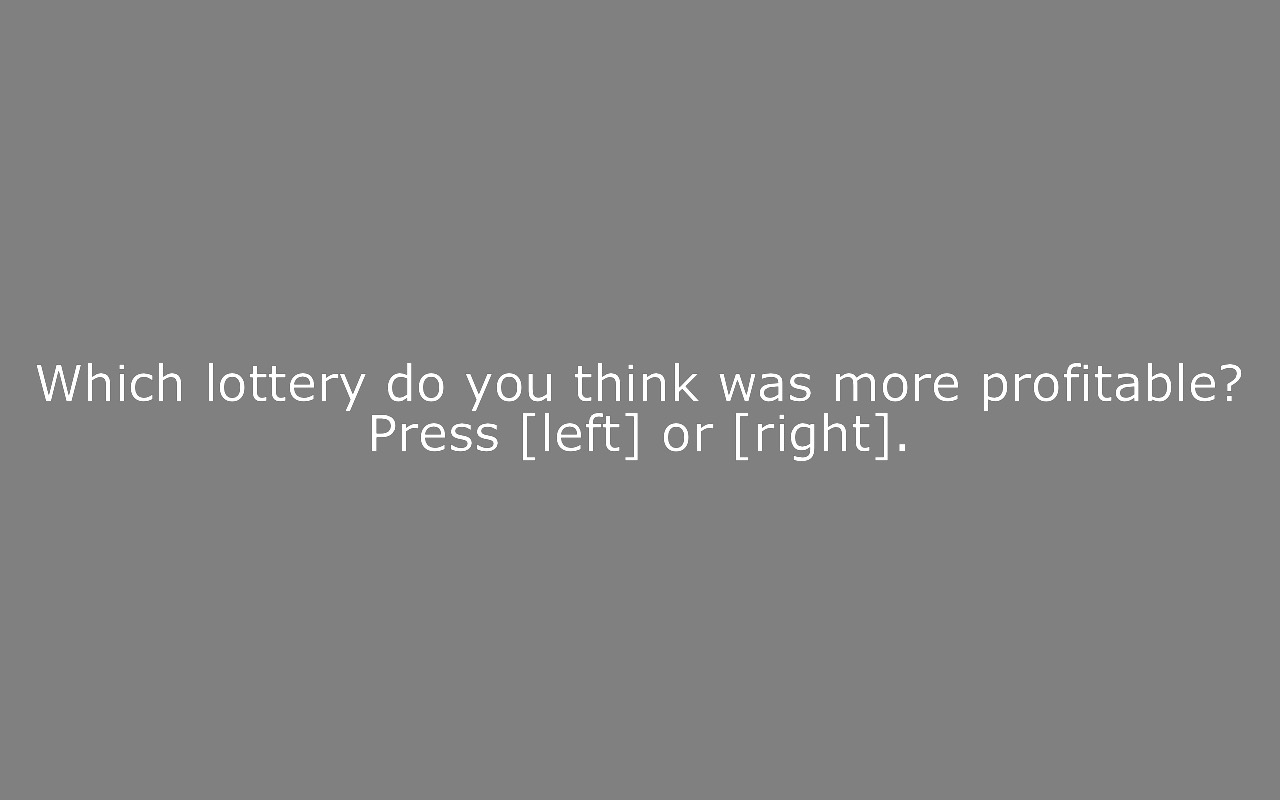
\includegraphics[width=\imgSize]{prefLot.jpg}};



% Drawing all nodes between pictures
\draw[->,thick] (lotShuffle) -- (trialCount)
    node [midway,fill=white] {$1250\pm250$ ms};

\draw[->,thick] (trialCount) -- (fixcross)
    node [midway,fill=white] {$1250\pm250$ ms};
    
\draw[->,thick] (fixcross) -- (outcome)
    node [midway,fill=white] {t depends on RT};
    
\draw[->,thick] (outcome) -- (earn)
    node [midway,fill=white] {$1250\pm250$ ms};
    
\draw[->,thick] (earn) -- (prefLot)
    node [midway,fill=white] {$1250\pm250$ ms};
    

% Inserting describing text next to pictures

\node at (4,0) [text width=\descrTextWidth, align=left, right] {The options [left] and [right] are shuffled once for each game.};

\node at (4,-4) [text width=\descrTextWidth, align=left, right] {Each trial starts with a counter indicating the current trial of all trials in the present game.};

\node at (4,-8) [text width=\descrTextWidth, align=left, right] {Once a fixation cross is shown, participants can select an option by clicking [left] or [right on the keyboard.]};

\node at (4,-12) [text width=\descrTextWidth, align=left, right] {Participants are provided with the outcome of their choice. Could also be a distractor trial, where participants need to press [space] as quickly as possible.};

\node at (4,-16) [text width=\descrTextWidth, align=left, right] {Once all trials of the present game have been finished, the overall earnings are displayed.};

\node at (4,-20) [text width=\descrTextWidth, align=left, right] {Lastly, participants are asked, which option they deemed more profitable.};


% Drawing the bent arrows 
\draw[->,thick] (outcome.west) to [out=180,in=180] node[text width=0.2\textwidth, midway, fill=white, align=center]{$1250\pm250$ ms \\ Increment trial counter and repeat until max trial is reached} (trialCount.west) ;


\draw[->,thick] (prefLot.west) to [out=180,in=180] node[text width=0.2\textwidth, midway, fill=white, align=center] {t depends on RT \\ Increment game counter and repeat until max game is reached} (lotShuffle.west);


\end{tikzpicture}
\end{center}
\end{figure}
\end{document}